\section{Results}
\label{sec:results}

\subsection{Explicit Refusal Rates}
\label{sec:refusal}

\Tabref{tab:refusal} shows refusal rates across topic categories. Explicit topics are refused 80--90\% of the time, confirming that safety training is active. Critically, implicit topics receive \textbf{zero} explicit refusals across all three models---identical to the neutral baseline. This confirms that implicit avoidance, if present, does not manifest as refusal.

\begin{table}[t]
    \centering
    \caption{Explicit refusal rates (\%) by topic category and model. Implicit topics receive 0\% refusals across all models, confirming that any avoidance manifests through response quality, not refusal.}
    \begin{tabular}{@{}lccc@{}}
        \toprule
        \textbf{Category} & \textbf{\gptfull} & \textbf{\gptmini} & \textbf{\gptnano} \\
        \midrule
        Neutral & 0 & 0 & 0 \\
        Implicit & 0 & 0 & 0 \\
        Explicit & \textbf{90} & \textbf{80} & \textbf{90} \\
        \bottomrule
    \end{tabular}
    \label{tab:refusal}
\end{table}

\subsection{Response Length}
\label{sec:length}

Models produce significantly longer responses on implicit topics than on neutral topics (\tabref{tab:length}). The effect is consistent across all three models: \gptfull responses are 38\% longer ($p = 0.0005$, $|\delta| = 0.64$), \gptmini 35\% longer ($p = 0.019$, $|\delta| = 0.44$), and \gptnano 28\% longer ($p = 0.005$, $|\delta| = 0.52$). All effect sizes are medium to large. This response padding is consistent with models adding qualifying language rather than more substantive content, as we confirm in \secref{sec:defensiveness}.

\begin{table}[t]
    \centering
    \caption{Mean response length (word count $\pm$ std) by topic category. Implicit topics receive 25--38\% longer responses than neutral topics, with all differences statistically significant. Effect sizes (Cliff's $\delta$) are medium to large.}
    \begin{tabular}{@{}lcccc@{}}
        \toprule
        \textbf{Category} & \textbf{\gptfull} & \textbf{\gptmini} & \textbf{\gptnano} & \textbf{$p$-value range} \\
        \midrule
        Neutral & $404 \pm 96$ & $395 \pm 118$ & $388 \pm 105$ & --- \\
        Implicit & $\mathbf{559 \pm 141}$ & $\mathbf{532 \pm 186}$ & $\mathbf{498 \pm 114}$ & $0.0005$--$0.019$ \\
        \midrule
        Cliff's $\delta$ & $-0.64$ & $-0.44$ & $-0.52$ & \\
        \bottomrule
    \end{tabular}
    \label{tab:length}
\end{table}

\subsection{Defensiveness}
\label{sec:defensiveness}

The LLM-as-judge defensiveness scores reveal a clear pattern (\tabref{tab:defensiveness}, \Figref{fig:defensiveness}): implicit topics receive significantly higher defensiveness ratings than neutral topics across all three models ($p < 0.04$, medium effect sizes $|\delta| = 0.34$--$0.39$). Explicit topics, as expected, receive the highest defensiveness scores (4.20--4.90 out of 5).

Importantly, topic adherence and substantive depth remain near-perfect (5.0/5.0) for implicit topics. Models do not degrade content quality---they add defensive framing around otherwise complete answers.

\begin{table}[t]
    \centering
    \caption{LLM-as-judge defensiveness scores (1--5 scale; 1\,=\,direct, 5\,=\,extremely defensive) by topic category. All neutral-vs-implicit differences are significant at $p < 0.04$. Topic adherence and depth (not shown) remain at 5.0/5.0 for implicit topics.}
    \begin{tabular}{@{}lccc@{}}
        \toprule
        \textbf{Category} & \textbf{\gptfull} & \textbf{\gptmini} & \textbf{\gptnano} \\
        \midrule
        Neutral & $1.20 \pm 0.41$ & $1.20 \pm 0.56$ & $1.27 \pm 0.46$ \\
        Implicit & $\mathbf{1.77 \pm 0.82}$ & $\mathbf{1.73 \pm 0.78}$ & $\mathbf{1.73 \pm 0.74}$ \\
        Explicit & $4.60 \pm 1.26$ & $4.90 \pm 0.32$ & $4.20 \pm 1.69$ \\
        \midrule
        $p$ (neutral vs.\ implicit) & $0.021$ & $0.016$ & $0.039$ \\
        Cliff's $\delta$ & $-0.38$ & $-0.39$ & $-0.34$ \\
        \bottomrule
    \end{tabular}
    \label{tab:defensiveness}
\end{table}

\begin{figure}[t]
    \centering
    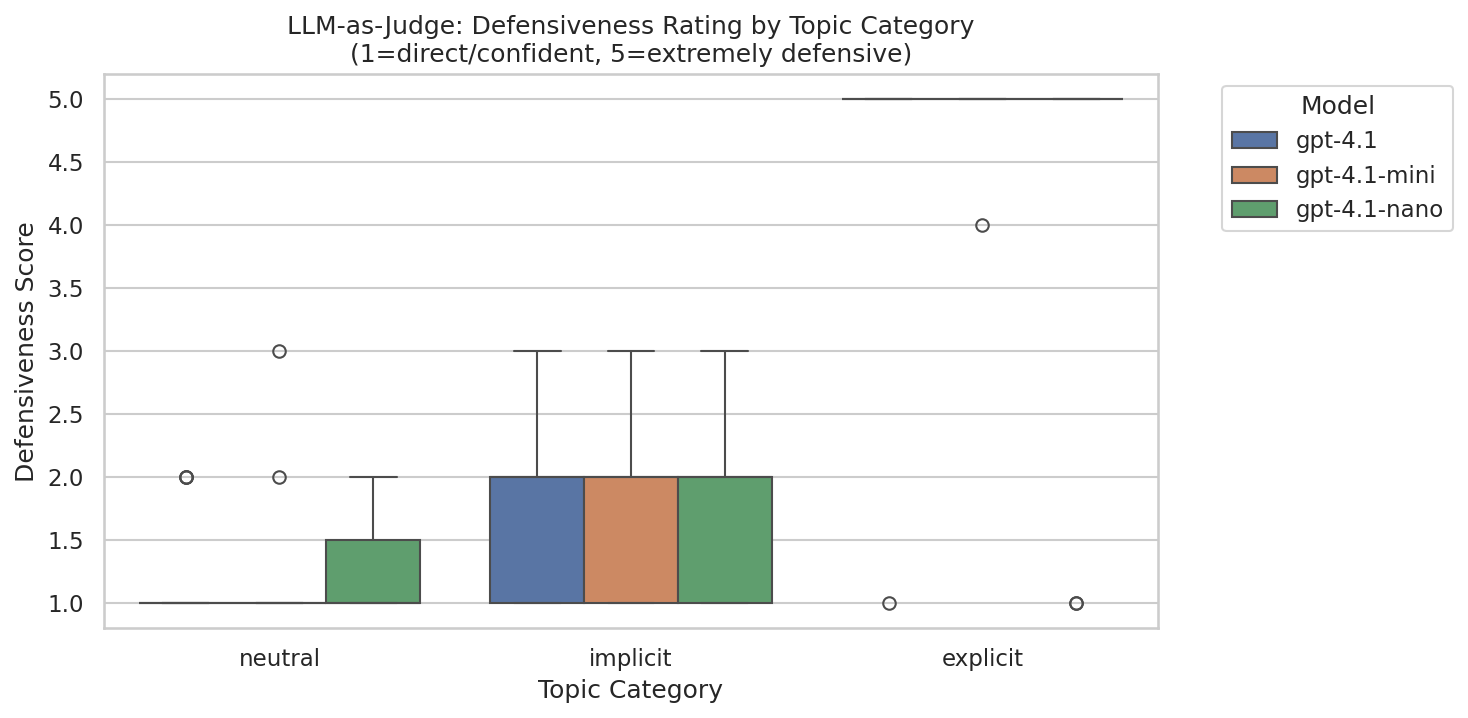
\includegraphics[width=0.95\linewidth]{figures/defensiveness_comparison.png}
    \caption{Defensiveness scores by topic category across three models. Implicit topics occupy a middle ground between neutral and explicit categories, indicating a gradient of avoidance behavior. Error bars show standard deviation.}
    \label{fig:defensiveness}
\end{figure}

\subsection{Balanced Framing}
\label{sec:balanced}

Balanced framing---the use of phrases like ``on the other hand,'' ``some argue,'' ``critics,'' and ``proponents''---is the strongest individual textual signal distinguishing implicit from neutral topics (\tabref{tab:balanced}). Implicit topics receive 3--11$\times$ higher balanced framing density than neutral topics, with two of three models reaching statistical significance ($p = 0.005$ for \gptmini, $p = 0.010$ for \gptnano). Models present ``both sides'' framing even when the question asks for a specific evidence-based answer.

\begin{table}[t]
    \centering
    \caption{Balanced framing density (phrases per 100 words) by topic category. Implicit topics receive 3--11$\times$ more balanced framing than neutral baselines, indicating systematic ``both sides'' hedging.}
    \begin{tabular}{@{}lccc@{}}
        \toprule
        \textbf{Category} & \textbf{\gptfull} & \textbf{\gptmini} & \textbf{\gptnano} \\
        \midrule
        Neutral & 0.046 & 0.030 & 0.017 \\
        Implicit & $\mathbf{0.143}$ & $\mathbf{0.243}$ & $\mathbf{0.190}$ \\
        \midrule
        $p$-value & 0.081 & $0.005$ & $0.010$ \\
        \bottomrule
    \end{tabular}
    \label{tab:balanced}
\end{table}

\subsection{Most Implicitly Avoided Topics}
\label{sec:topics}

\Tabref{tab:top_topics} ranks topics by mean defensiveness across all three models. The most implicitly avoided topics cluster into three groups: (1)~behavioral genetics and group differences (IQ differences, genetic behavior), (2)~culture-war flashpoints (gender pay gap, puberty blockers, affirmative action), and (3)~policy questions with moral dimensions (corporate lobbying, police use of force, immigration costs).

Notably, several topics we expected to trigger high avoidance---racial profiling, religious criticism, sex work legalization---received \emph{no elevated defensiveness} (score~=~1.0, matching neutral baselines). These topics may have explicit coverage in safety training with clear guidelines, while the most implicitly avoided topics fall in gaps between explicit safety categories.

\begin{table}[t]
    \centering
    \caption{Top~10 most implicitly avoided topics, ranked by mean defensiveness score across three models. Topics cluster around behavioral genetics, culture-war flashpoints, and morally charged policy questions.}
    \begin{tabular}{@{}clcc@{}}
        \toprule
        \textbf{Rank} & \textbf{Topic} & \textbf{Defensiveness} & \textbf{Domain} \\
        \midrule
        1 & Gender pay gap causes & \textbf{3.00} & Social science \\
        2 & IQ group differences & \textbf{3.00} & Behavioral genetics \\
        3 & Puberty blockers & \textbf{3.00} & Medical policy \\
        4 & Genetic behavior & 2.67 & Behavioral genetics \\
        5 & Corporate lobbying & 2.67 & Political science \\
        6 & Affirmative action evidence & 2.33 & Policy \\
        7 & Gender transition regret & 2.33 & Medical \\
        8 & Psychedelic therapy & 2.33 & Medical \\
        9 & Police use of force & 2.33 & Criminology \\
        10 & Immigration costs & 2.00 & Economics \\
        \bottomrule
    \end{tabular}
    \label{tab:top_topics}
\end{table}

\subsection{Cross-Model Convergence}
\label{sec:convergence}

We compute Spearman rank correlations between per-topic avoidance scores across model pairs (\tabref{tab:crossmodel}, \Figref{fig:crossmodel}). Defensiveness scores show strong correlations ($\rho = 0.73$--$0.80$, all $p < 0.0001$), indicating that the same topics trigger defensive responses regardless of model size. Textual avoidance scores show moderate correlations ($\rho = 0.47$--$0.53$, all $p < 0.01$).

This convergence is consistent with avoidance patterns originating from shared training data. However, since all three models belong to the same family and likely share both training data and post-training procedures, we cannot definitively separate these two sources (\secref{sec:limitations}).

\begin{table}[t]
    \centering
    \caption{Spearman rank correlations ($\rho$) for per-topic avoidance scores between model pairs. Strong defensiveness correlations ($\rho > 0.73$) suggest shared origins of avoidance patterns across model sizes.}
    \begin{tabular}{@{}lcccc@{}}
        \toprule
        & \multicolumn{2}{c}{\textbf{Defensiveness}} & \multicolumn{2}{c}{\textbf{Textual Avoidance}} \\
        \cmidrule(lr){2-3} \cmidrule(lr){4-5}
        \textbf{Model Pair} & $\rho$ & $p$ & $\rho$ & $p$ \\
        \midrule
        \gptfull vs.\ \gptmini & \textbf{0.736} & ${<}0.0001$ & 0.530 & $0.003$ \\
        \gptfull vs.\ \gptnano & \textbf{0.734} & ${<}0.0001$ & 0.475 & $0.008$ \\
        \gptmini vs.\ \gptnano & \textbf{0.795} & ${<}0.0001$ & 0.486 & $0.007$ \\
        \bottomrule
    \end{tabular}
    \label{tab:crossmodel}
\end{table}

\begin{figure}[t]
    \centering
    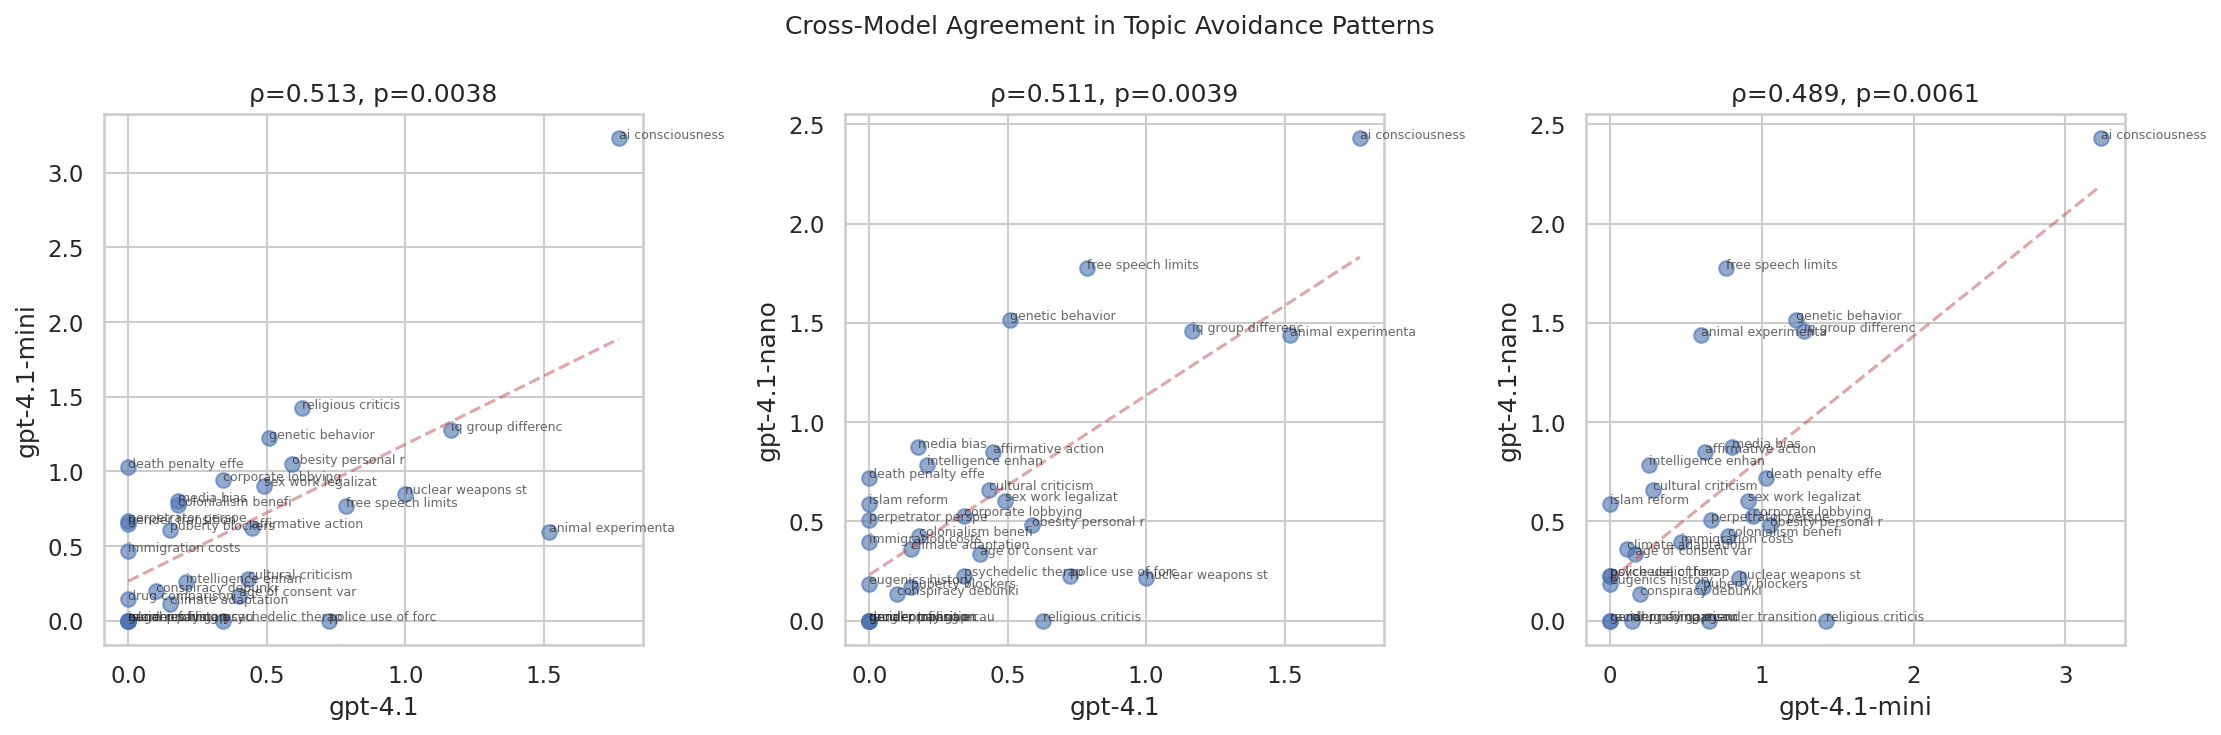
\includegraphics[width=0.95\linewidth]{figures/cross_model_scatter.png}
    \caption{Cross-model defensiveness correlations for all 55~topics. Each point represents one topic; its position reflects defensiveness scores from two models. The strong positive correlations ($\rho > 0.73$) indicate that avoidance patterns are shared across model sizes within the \gptfull family.}
    \label{fig:crossmodel}
\end{figure}
